\chapter{Opis projektnog zadatka}
		

Cilj projektnog zadatka je izrada web aplikacije „Zamjena soba“ koja omogućuje studentima koji žive u studentskim domovima da s lakoćom zamijene sobu s nekim drugim zainteresiranim studentom. Trenutno se ovaj problem rješava usmenim dogovorom studenata ili, još češće, preko društvenih mreža. Nakon toga studenti moraju ići u nadležni Studentski centar da im se odobri zamjena, što također komplicira cijeli postupak. Zamjena soba na ovaj način jako je neorganizirana te zbog nemogućnosti pregleda svih soba koje su dostupne za zamjenu ponekad se dogodi da studenti ne uspiju pronaći idealno rješenje.  \\
		
		Aplikacija „Zamjena soba“ predstavlja soluciju za navedene probleme. Prilikom ulaska u aplikaciju otvara se početna stranica na kojoj se nalaze predani oglasi iz različitih gradova i studentskih domova. Neregistrirani korisnik može gledati oglase, ali preduvjet za korištenje bilo koje druge funkcionalnosti je registracija i/ili prijava u sustav. Neregistriranom korisniku omogućeno je prijavljivanje u sustav s postojećim računom ili izradom novog računa (registracija). Ako se korisnik prijavljuje s postojećim računom potrebno je unijeti korisničko ime i lozinku nakon čega sustav provjera oba podatka i prijavljuje korisnika u sustav. Za kreiranje novog računa potrebno je unijeti:  
		
		\begin{packed_item}
			\item ime
			\item email
			\item JMBAG
			\item korisničko ime
			\item lozinku
		\end{packed_item}
		
		
		Korisnici pri registraciji dobivaju ulogu Studenta, a djelatnicima SC-a su korisnički podaci uneseni direktno u bazu podataka te ne trebaju vršiti registraciju u sustav. \\
		\underbar{Studentu} se prilikom prijave u aplikaciju otvara početna stranica na kojoj se nalaze predani oglasi drugih studenata. Student može otići na stranicu „Predaj oglas“ na kojoj navodi značajke svojeg mjesta u domu: 
		
		\begin{packed_item}
			\item grad
			\item dom
			\item paviljon
			\item kategorija sobe
			\item kat
			\item najbliža menza
		\end{packed_item}

te također navodi značajke mjesta u domu koje želi. Prilikom izrade oglasa za vlastito mjesto mora popuniti sve značajke, a za mjesto koje želi može ostaviti jednu ili više značajki prazno (ako mu ta značajka nije bitna). Student sve svoje oglase može vidjeti na stranici „Moji oglasi“. Tamo se nalaze aktivni i neaktivni oglasi, a aktivni oglasi mogu se uređivati (npr. student može promijeniti značajke domskog mjesta koje želi dobiti). U jednom trenutku samo jedan korisnikov oglas može biti aktivan. Nakon što student unese značajke domskog mjesta koje želi, početna stranica mu se mijenja. Prikazuju se oglasi osoba koje žele onu sobu u domu koju je student oglasio te koje nude sobu koja ima značajke koje je student označio. Također na početnoj stranici su dostupne i sobe koje su u tzv. lancima razmjene (sobe za koje se mogu ostvariti zamjene s tri ili više studenata, a da svatko dobije što želi). Kad se pojave novi oglasi koji odgovaraju navedenim kriterijima, osim što će se pojaviti na početnoj stranici, student će također dobiti obavijest mailom: „Imate nove kandidate za zamjenu sobe u domu!“ s linkom za pregled istih. Sve dostupne oglase student može “lajkati“ , i to po stupnjevima:

	\begin{packed_item}

			\item[] \begin{packed_enum}
				\item sviđa mi se
				\item sviđa mi se jako
				\item to je to
			\end{packed_enum}
			
		\end{packed_item}
		
ili označiti „Ne prikazuj više ovaj oglas“. Kada su obje uključene strane „lajkale“ zamjenu soba, oba studenta bit će obaviještena mailom u kojem će se od njih tražiti da daju konačnu potvrdu zamjene soba. Student će dobiti link u mailu te klikom na taj link otvorit će se stranica za zamjenu na kojoj će student imati mogućnost pregledati zamjenu i prihvatiti željenu sobu. Oba studenta moraju prihvatiti željenu sobu da bi se zamjena dogodila. Nakon što oba studenta prihvate zamjenu, djelatniku SC-a ta zamjena biti će vidljiva i moći će je evidentirati u Studentskom centru.\\

Djelatniku SC-a prilikom prijave u sustav otvaraju se sve zaključane zamjene za studentske domove koji se nalaze u gradu za koji je taj Studentski centar nadležan. Nakon što djelatnik SC-a pogleda neku zamjenu i zabilježi je u sustav SC-a, može je označiti kao obavljenu te se kasnije obavljene zamjene više nigdje ne prikazuju.\\


Rješenje je trenutno izvedeno samo za državne studentske domove, ali moglo bi se prilagoditi za sve studentske domove (privatne i državne) , privatne sobe i stanove u kojima stanuju studenti.\\

Projektni zadatak mogao bi se nadograditi na više načina. Jedan od načina je da student prilikom unosa željenih značajki u domu ima mogućnost navođenja 3 ili 5 tipova soba koje ga zanimaju  tako da značajke mjesta u domu koje ga najviše zanima stavi na prvo mjesto. Na taj način bi student dobio više izbora prilikom traženja sobe za zamjenu. \\

Ovaj projekt uvelike bi olakšao i ubrzao zamjenu soba studentima. Neka sveučilišta u svijetu već su razvila aplikacije koje omogućavaju studentima slične mogućnosti. Jedan primjer aplikacije je aplikacija Sveučilišta u Bostonu koja svojim studentima nudi mogućnost oglašavanja vlastite i pronalaska željene sobe. Za razliku od naše aplikacije koja nudi mogućnost korisnicama da sami pregledavaju oglase i označavaju one koje im se sviđaju, aplikacija Sveučilišta u Bostonu nema tu mogućnost. Sustav sam pronalazi moguće zamjene i šalje ih na mail zainteresiranim studentima koji nakon toga trebaju provesti potvrdu. \\

Slika 2.1 prikazuje stranicu aplikacije za zamjenu soba Sveučilišta u Bostonu na kojoj je prikazana ponuda za zamjenu soba koju je student dužan potvrditi ukoliko želi da se zamjena ostvari. Ova funkcionalnost implementirana je i u našoj aplikaciji.

%unos slike
		\begin{figure}[H]
			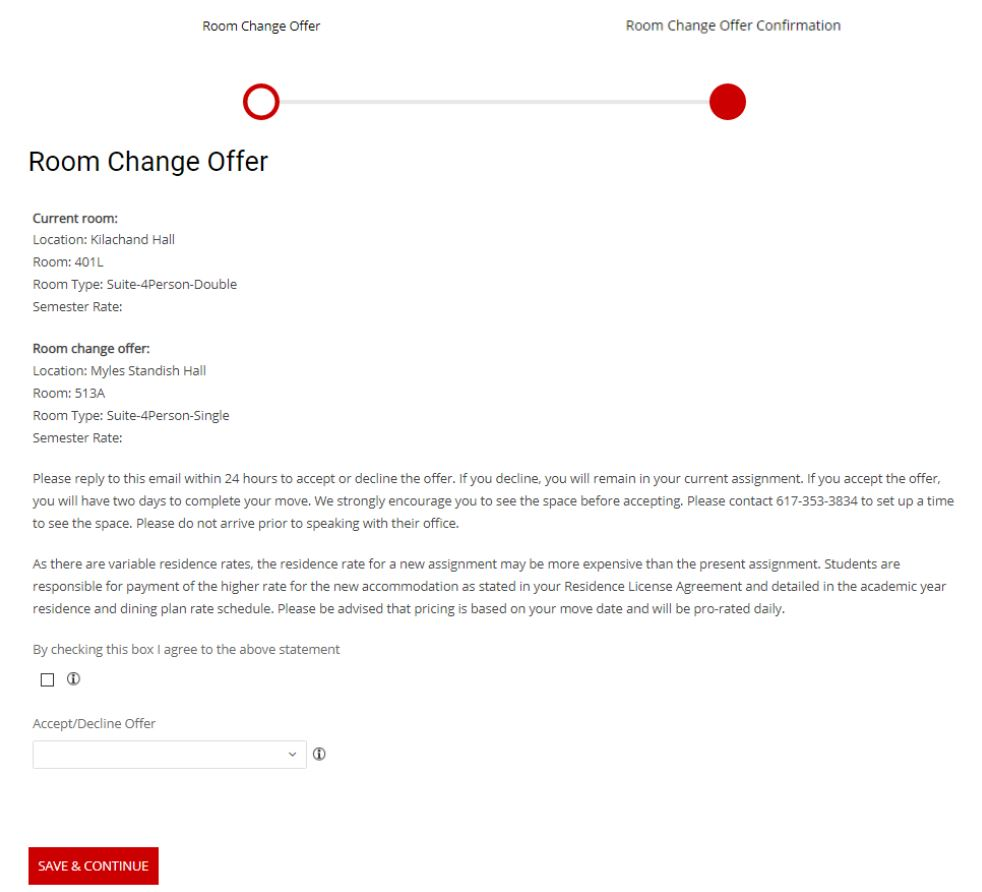
\includegraphics[scale=0.4]{slike/pic1.JPG} %veličina slike u odnosu na originalnu datoteku i pozicija slike
			\centering
			\caption{Aplikacija za zamjenu soba Sveučilišta u Bostonu}
			\label{fig:promjene1}
		\end{figure}

	